\documentclass[conf]{new-aiaa}
%\documentclass[journal]{new-aiaa} for journal papers
\usepackage[utf8]{inputenc}
\usepackage{float}

\usepackage{graphicx}
\usepackage{amsmath}
\usepackage[version=4]{mhchem}
\usepackage{siunitx}
\usepackage{longtable,tabularx}
\setlength\LTleft{0pt} 

\title{AE 598-RL HW1 Report}

\author{Gokul Puthumanaillam (gokulp2}
\affil{Department of Aerospace Engineering, University of Illinois Urbana-Champaign}

\begin{document}

\maketitle


\section{Introduction}
This report documents the generated graphs for the following algorithms in the Grid World and the Discrete Pendulum (in a tabular setting):
\begin{enumerate}
    \item Value Iteration: Grid World
    \item Policy Iteration: Grid World
    \item SARSA: Grid World and Discrete Pendulum
    \item QLearning: Grid World and Discrete Pendulum
\end{enumerate}
\section{Hyperparameters:}
\subsection{Grid World}
\subsubsection{Value Iteration and Policy Iteration}
\begin{enumerate}
    \item Max Number of episodes: 5000
    \item $\gamma$: 0.95
    \item $\theta$=1e-6
\end{enumerate}


\subsubsection{SARSA}
\begin{enumerate}
    \item Max Number of episodes: 5000
    \item $\gamma$: 0.95
    \item $\theta$: 1e-6
    \item $\epsilon$: 0.1
\end{enumerate}

\subsubsection{QLearning}
\begin{enumerate}
    \item Max Number of episodes: 5000
    \item $\gamma$: 0.95
    \item $\theta$: 1e-6
    \item $\epsilon$: 0.1
\end{enumerate}

\subsection{Discrete Pendulum}

\subsubsection{SARSA}
\begin{enumerate}
    \item Max Number of episodes: 700
    \item $\gamma$: 0.95
    \item $\theta$: 1e-6
    \item $\epsilon$: 0.1
\end{enumerate}

\subsubsection{QLearning}
\begin{enumerate}
    \item Max Number of episodes: 700
    \item $\gamma$: 0.95
    \item $\theta$: 1e-6
    \item $\epsilon$: 0.1
\end{enumerate}


\section{Plots}
\subsection{Grid World}
\begin{figure}[H]
\centering
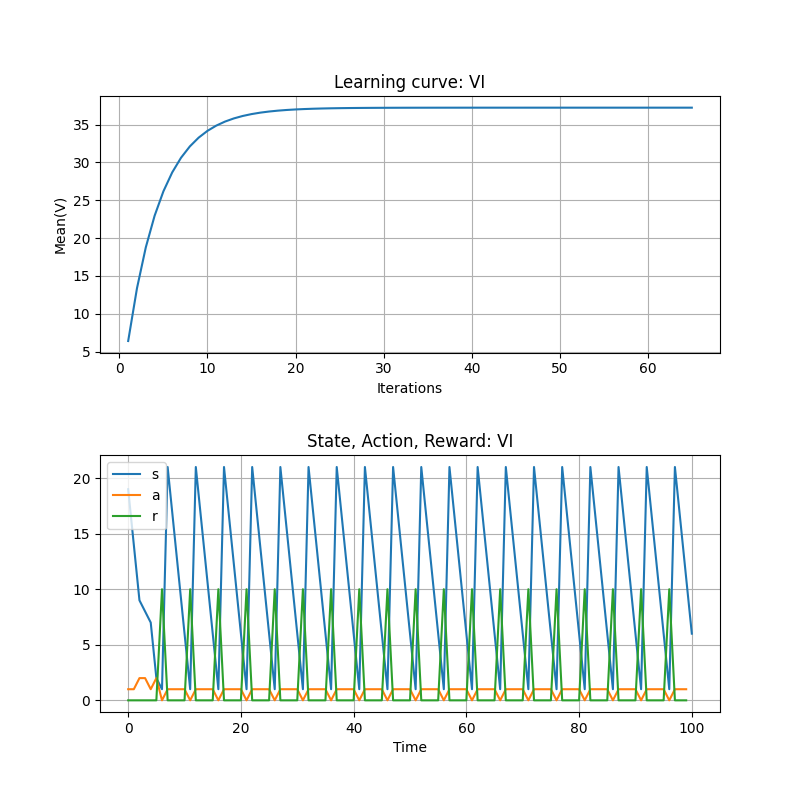
\includegraphics[width=30pc]{figs/gw/learning_and_trajectory_vi.png}
\caption{Plots showing the learning curve for Value Iteration and the State, Action, Rewards}
\label{fig_env1}
\end{figure}

\begin{figure}[H]
\centering
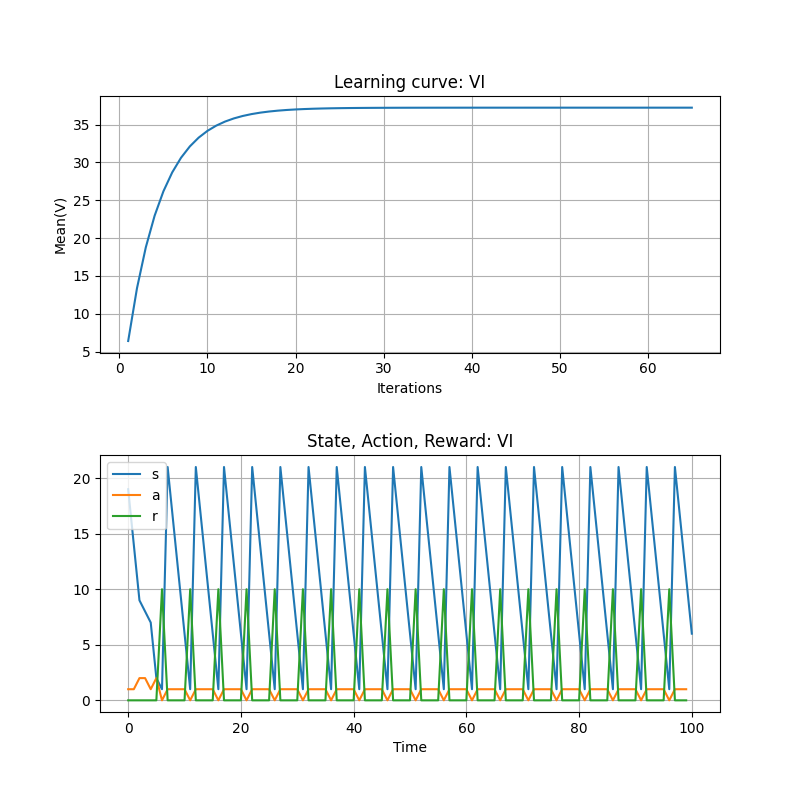
\includegraphics[width=30pc]{figs/gw/learning_and_trajectory_vi.png}
\caption{Plots showing the learning curve for Policy Iteration and the State, Action, Rewards}
\label{fig_env1}
\end{figure}

\begin{figure}[H]
\centering
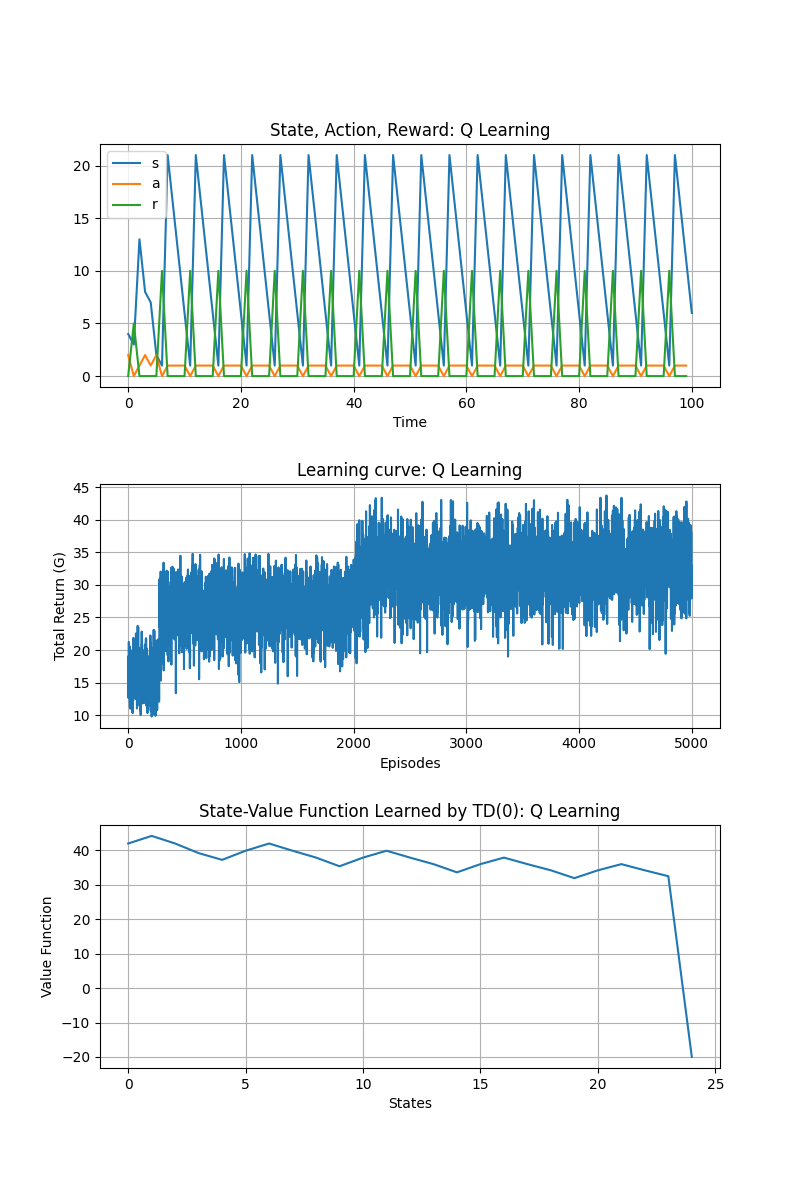
\includegraphics[width=30pc]{figs/gw/qlearning_plots.png}
\caption{Plots for QLearning: (a)State, Action, Reward (b) Learning Curve (c) State Value Function Estimation using TD(0)}
\label{fig_env1}
\end{figure}



\begin{figure}[H]
\centering
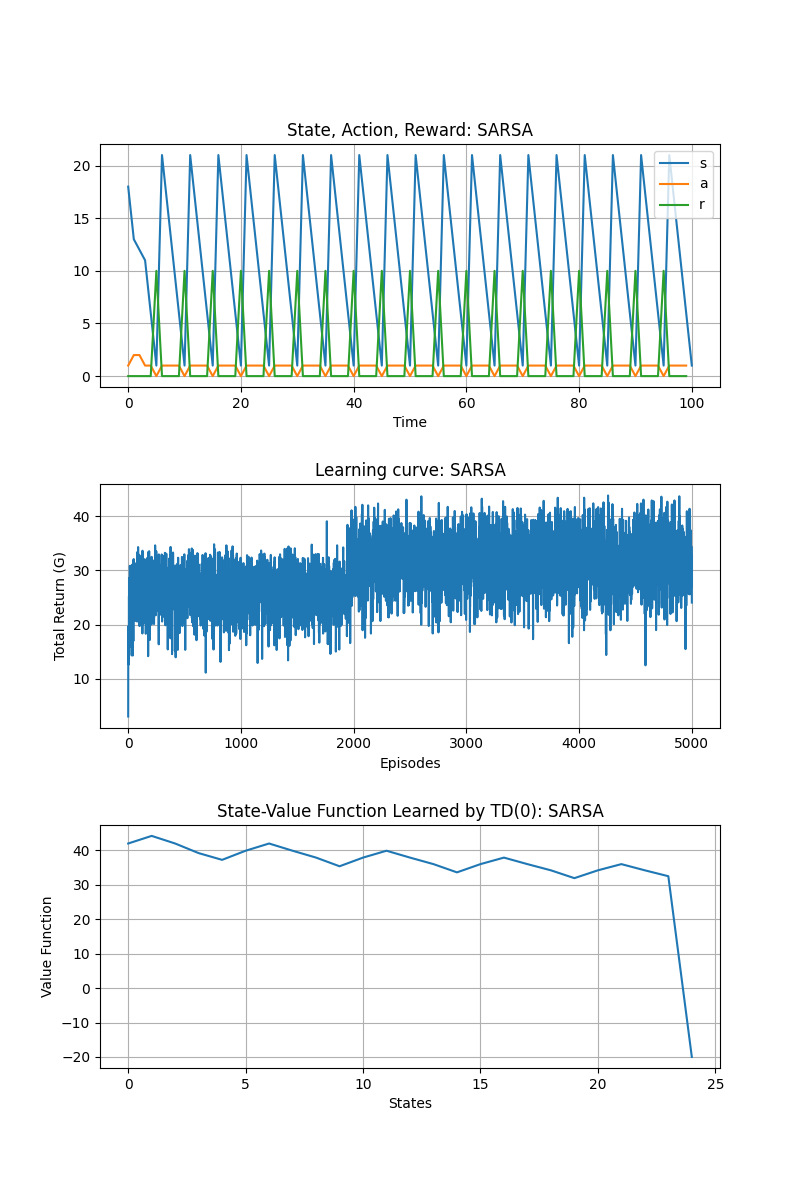
\includegraphics[width=30pc]{figs/gw/sarsa_plots.png}
\caption{Plots for SARSA: (a)State, Action, Reward (b) Learning Curve (c) State Value Function Estimation using TD(0)}
\label{fig_env1}
\end{figure}




\begin{figure}[H]
\centering
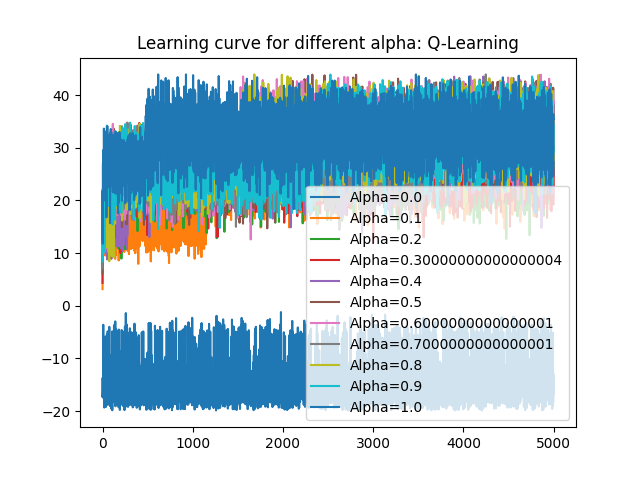
\includegraphics[width=30pc]{figs/gw/alpha_sweep_qlearning.png}
\caption{Learning Curve for different Alpha: QLearning}
\label{fig_env1}
\end{figure}

\begin{figure}[H]
\centering
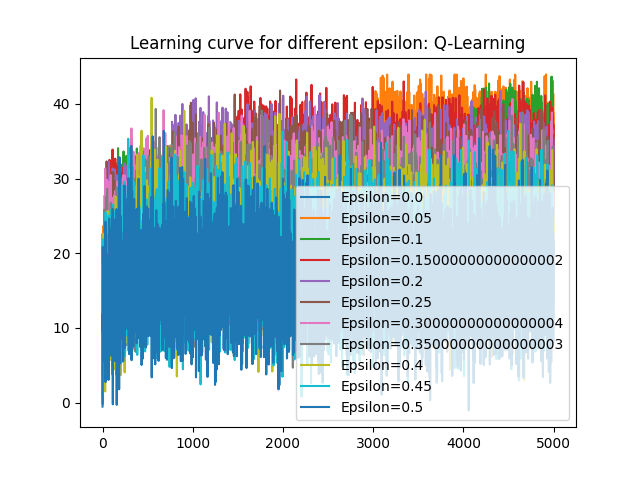
\includegraphics[width=30pc]{figs/gw/epsilon_sweep_qlearning.png}
\caption{Learning Curve for different Epsilon: QLearning}
\label{fig_env1}
\end{figure}




\begin{figure}[H]
\centering
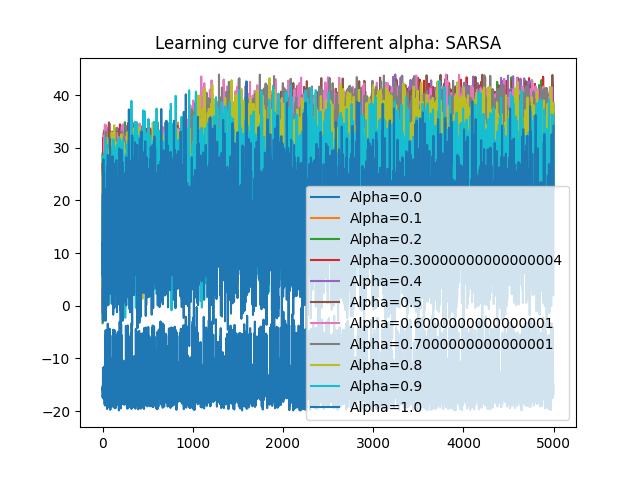
\includegraphics[width=30pc]{figs/gw/alpha_sweep_SARSA.png}
\caption{Learning Curve for different Alpha: SARSA}
\label{fig_env1}
\end{figure}

\begin{figure}[H]
\centering
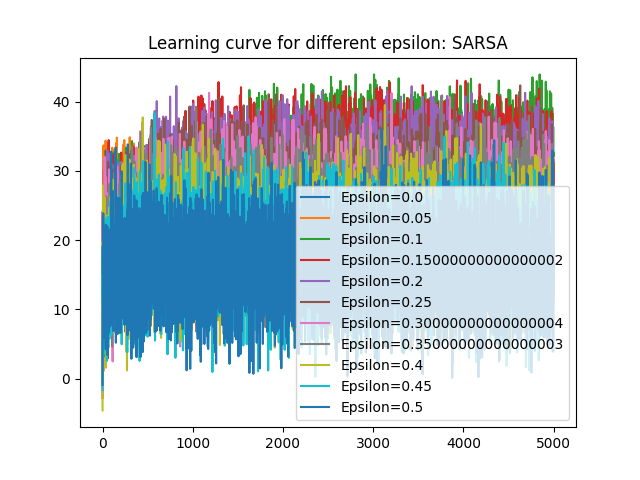
\includegraphics[width=30pc]{figs/gw/epsilon_sweep_SARSA.png}
\caption{Learning Curve for different Epsilon: SARSA}
\label{fig_env1}
\end{figure}





\newpage
\subsection{Discrete Pendulum}


\begin{figure}[H]
\centering
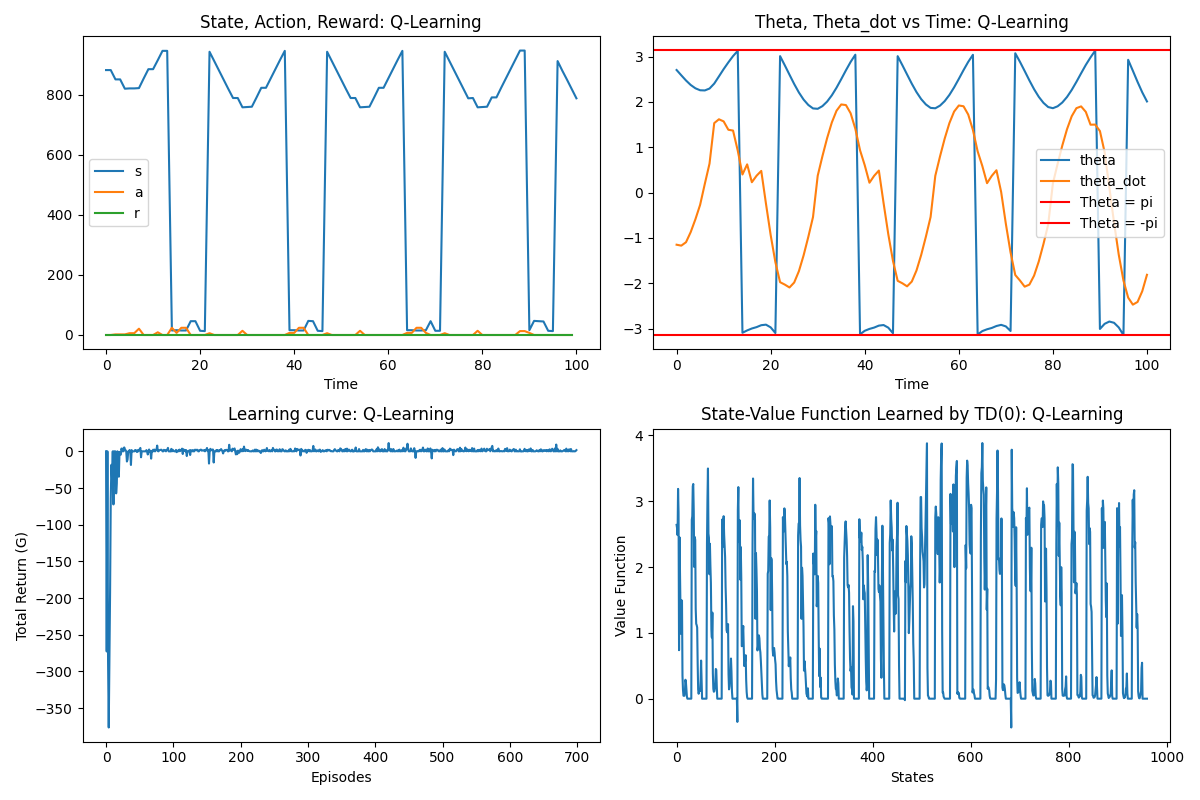
\includegraphics[width=30pc]{figs/pen/subplots_qlearning.png}
\caption{Plots for QLearning: (a)State, Action, Reward (b) Theta, Theta dot vs time(c) Learning Curve (d) State Value Function Estimation using TD(0)}
\label{fig_env1}
\end{figure}


\begin{figure}[H]
\centering
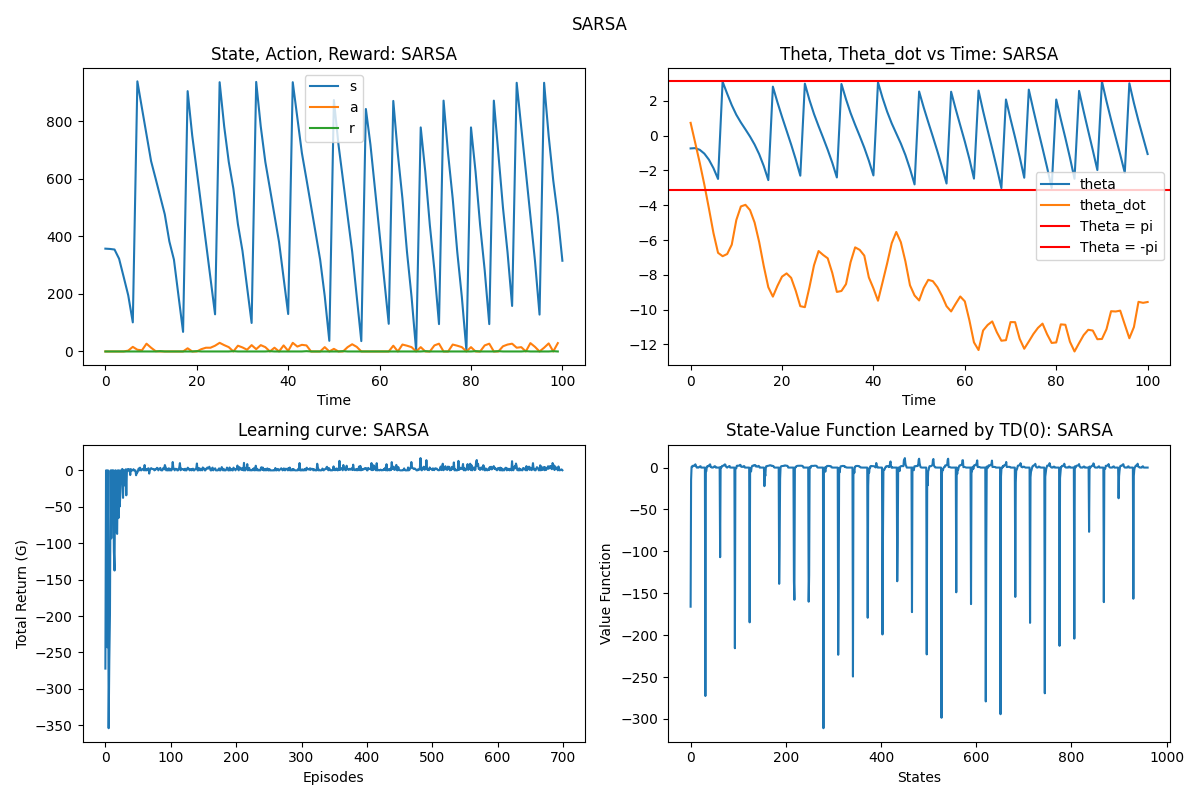
\includegraphics[width=30pc]{figs/pen/sarsa_plots.png}
\caption{Plots for SARSA: (a)State, Action, Reward (b) Theta, Theta dot vs time(c) Learning Curve (d) State Value Function Estimation using TD(0)}
\label{fig_env1}
\end{figure}




\begin{figure}[H]
\centering
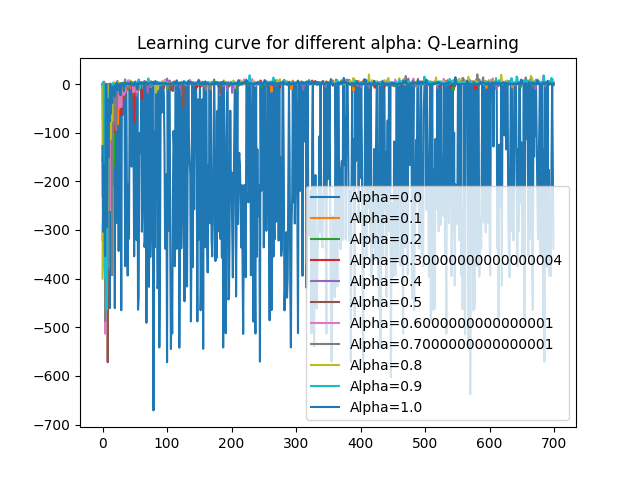
\includegraphics[width=30pc]{figs/pen/alpha_sweep_qlearning.png}
\caption{Learning Curve for different Alpha: QLearning}
\label{fig_env1}
\end{figure}


\begin{figure}[H]
\centering
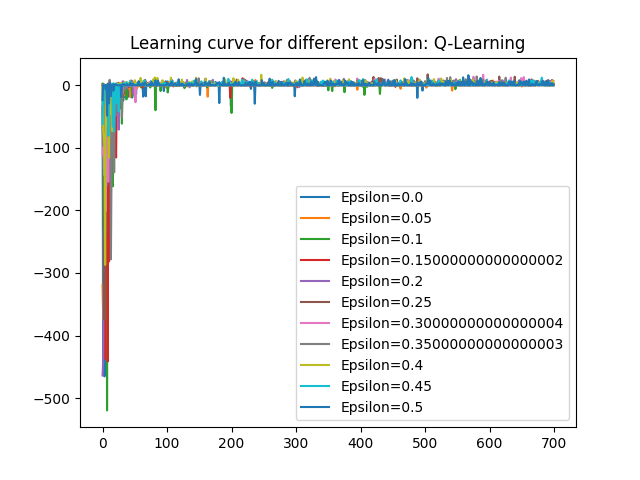
\includegraphics[width=30pc]{figs/pen/epsilon_sweep_qlearning.png}
\caption{Learning Curve for different Epsilon: QLearning}
\label{fig_env1}
\end{figure}


\begin{figure}[H]
\centering
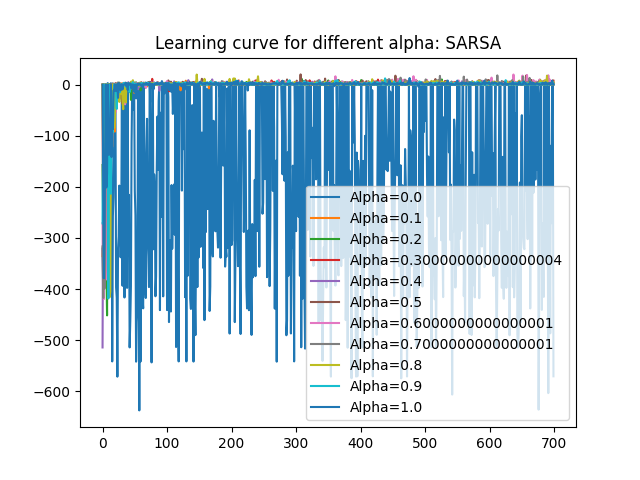
\includegraphics[width=30pc]{figs/pen/alpha_sweep_SARSA.png}
\caption{Learning Curve for different Alpha: SARSA}
\label{fig_env1}
\end{figure}


\begin{figure}[H]
\centering
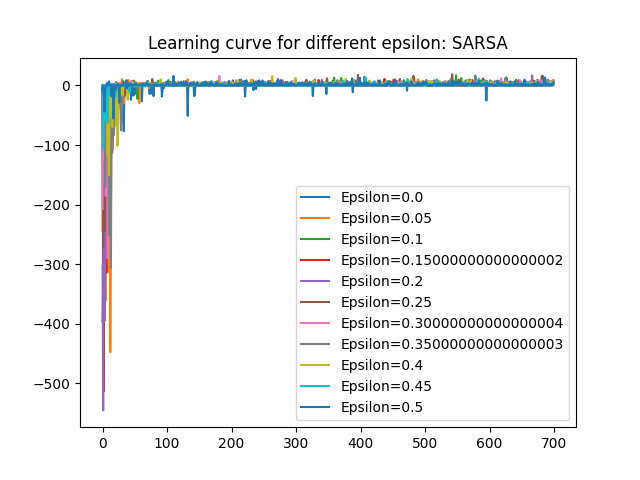
\includegraphics[width=30pc]{figs/pen/epsilon_sweep_SARSA.png}
\caption{Learning Curve for different Epsilon: SARSA}
\label{fig_env1}
\end{figure}


\end{document}
